\section{Multi-armed Bandits}


\subsection{Exercise 2.1}
Define $a_1$, $a_2$ as the two actions that can be taken, $\varepsilon$ as the probability of selecting a random action, and $r$ as a randomly generated number $\in [0,1]$. 
\begin{equation}
    \text{action} = 
    \begin{cases}
        \text{random choice of $a_1$ or $a_2$} & \text{if } r < \varepsilon \\
        \text{greedy choice} & \text{if } r \geq \varepsilon
        \end{cases}
\end{equation}

if $\varepsilon$ is 0.5, there is a 0.5 probability of taking the greedy choice and 0.5 probability of picking the random choice. The random choice has two actions, therefore there is a choice of picking $a_1$ or $a_2$ with 0.25 prob each. $0.25 + 0.50 = 0.75$, therefore the probability of the greedy action getting selected is 0.75

\subsection{Exercise 2.2}
$k$-armed bandits with $k$ = 4. $\varepsilon$-greedy algorithm setting $Q_1(a) = 0 \text{ }\forall a$.
Sample a trajectory $(a_1,r_1,a_2,\dots) \text{ } as \text{ } (1,-1, 2,1, 2,-2,2,2,3,0)$

\begin{itemize}
  \item $A_1 = 1$, Greedy (tie broken) or random
  \item $A_2 = 2$, Greedy (tie broken) or random
  \item $A_3 = 2$, Greedy or random
  \item $A_4 = 2$, Must have been random because average reward of $a_2$ is now $-1/2$
  \item $A_5 = 3$, Greedy (tie broken) or random
\end{itemize}

\subsection{Exercise 2.3}
In the long run, the $\varepsilon = 0.01$ will perform the best. On average, it will pick the optimal action more frequently while still sampling each action an infinite number of times. In the long run, as $Q(a) \approx q_*(a), $ $\varepsilon= 0.01$ will sample the optimal action 99.1\% of the time,  whereas $\varepsilon = 0.1$ will sample the optimal action 91\% of the time, resulting in a smaller frequency of the optimal action being picked and a smaller total reward over the long run. 

\subsection{Exercise 2.4}
Deriving the weighting on prior reward for general case $\alpha_n \not= \alpha$

\begin{gather}
  Q_{n+1} = Q_n + \alpha_n[R_n - Q_n] \\
  Q_{n+1} = \alpha_nR_n + (1-\alpha_nQ_n) \\
  Q_{n+1} = \alpha_nR_n + (1-\alpha_n[\alpha_{n-1}R_{n-1} + (1-\alpha_{n-1})Q_{n-1}]) \\
  Q_{n+1} = \alpha_nR_n + (1-\alpha_n)\alpha_{n-1}R_{n-1} + (1-\alpha_n)(1-\alpha_{n-1})Q_{n-1} \\
  Q_{n+1} = Q_1\prod\limits_{i=1}^n(1-\alpha_i) + \sum\limits_{i=1}^nR_i\alpha_i\prod\limits_{j=i+1}^n(1-\alpha_j)
\end{gather}

\subsection{Exercise 2.5}
Completed in code


\begin{figure}[htbp]
  \centering
  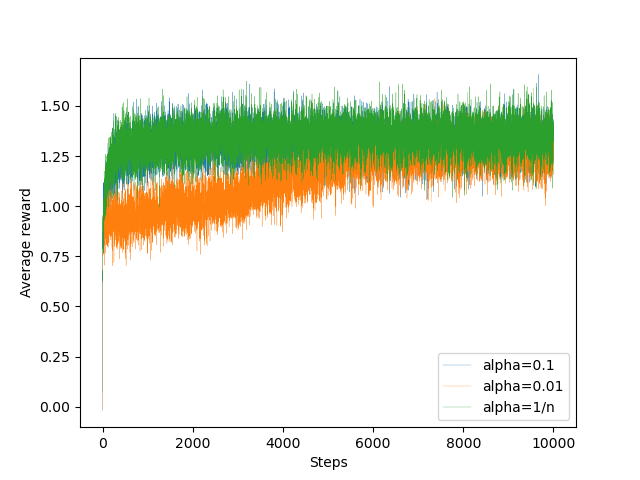
\includegraphics[width=0.5\textwidth]{../../code/figures/exercise2_5a.png}
\end{figure}

\begin{figure}[htbp]
  \centering
  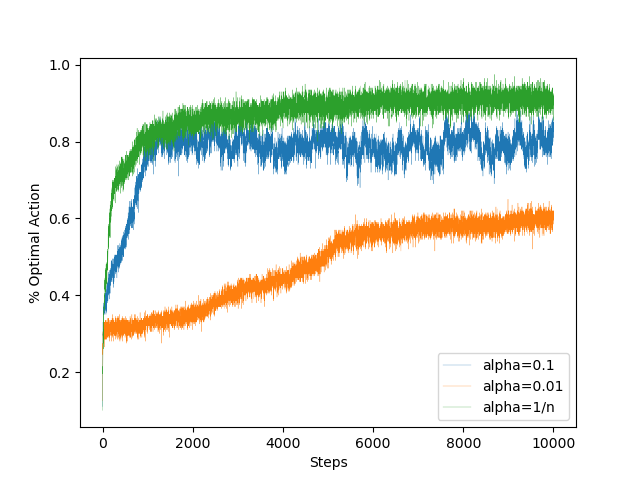
\includegraphics[width=0.5\textwidth]{../../code/figures/exercise2_5b.png}
\end{figure}

\subsection{Exercise 2.6}
Optimism will cause every option to look appealing until the option has been sampled enough times. If the option that is appealing happens to be an optimal choice, the decay of the Q value will be slower than that of the other choices.

\subsection{Exercise 2.7}
$\bar{o}_0 = 0$, therefore $\bar{o}_1 = 0 + \alpha(1-0) = \alpha$. $\beta_1 = \alpha/\alpha = 1$. Using the equation derived at the end of exercise 2.4,  $Q_1\prod\limits_{i=1}^n(1-\alpha_i)$ is 0 since $\alpha_1$ is 0. $Q_n$ does not include $Q_1$ so it is without initial bias.

\subsection{Exercise 2.8}
In the UCB algorithm, each arm must be sampled once. Each arm that has not been pulled ($N_t(a) = 0$), is classified as a maximizing action and will likely be pulled in the first $|A|$ actions. Since each arm has been sampled, on average, the optimal action will be the most appealing as it will provide the most reward in the long run. Therefore, each action will be made once and then the best seeming action is most likely to be selected.

\subsection{Exercise 2.9}